\section{引言}
\frame
{
	\frametitle{\secname~ }
	\begin{block}{选题背景与意义}
		是什么,为什么?
	\end{block}
	\begin{block}{国内外研究现状}
		主流方法是什么?
	\end{block}
	\begin{block}{本文的工作}
		我提出的方法是什么,有什么不同?
	\end{block}
}

\subsection*{选题背景与意义}
\frame{
	\frametitle{图像语义分割问题的定义}
	\begin{block}{}
		图像语义分割 (Semantic Image Segmentation) 是根据物体类别把图像分成若干个有意义的区域,并为不同的区域标注其所属标签的视觉任务。
	\end{block}
	\begin{figure}%文中的Grid-LSTM模型做的语义图像分割的例子
		\centering
		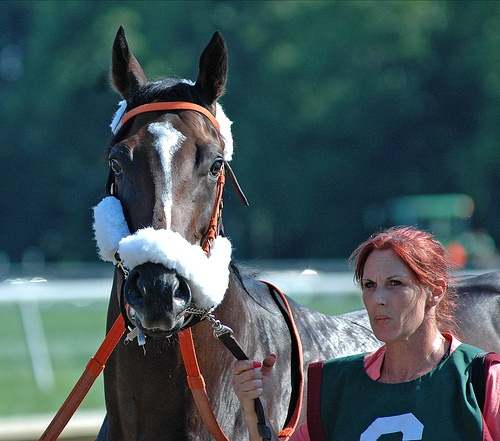
\includegraphics[width=.2\textwidth,height=.15\textwidth]{image/chap04/example/2007_000799.jpg}
		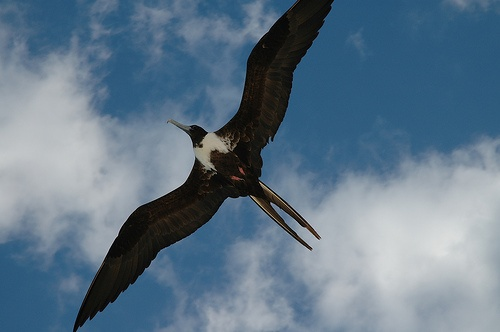
\includegraphics[width=.2\textwidth,height=.15\textwidth]{image/chap04/example/2007_002094.jpg}
		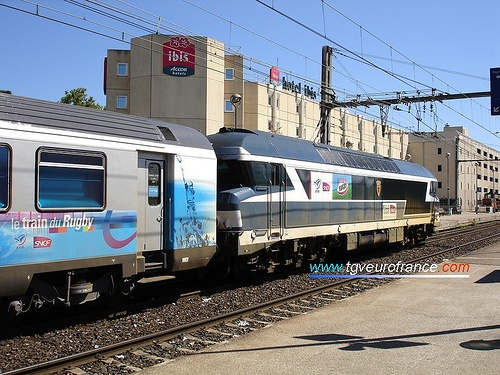
\includegraphics[width=.2\textwidth,height=.15\textwidth]{image/chap04/example/2007_004483.jpg}
		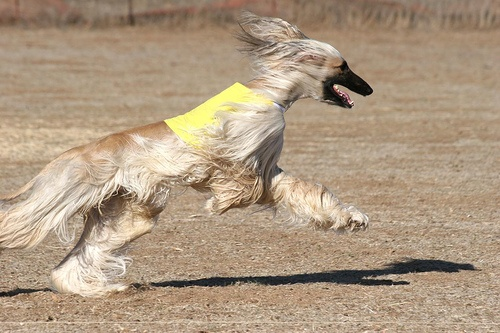
\includegraphics[width=.2\textwidth,height=.15\textwidth]{image/chap04/example/2007_003194.jpg}
		\\
		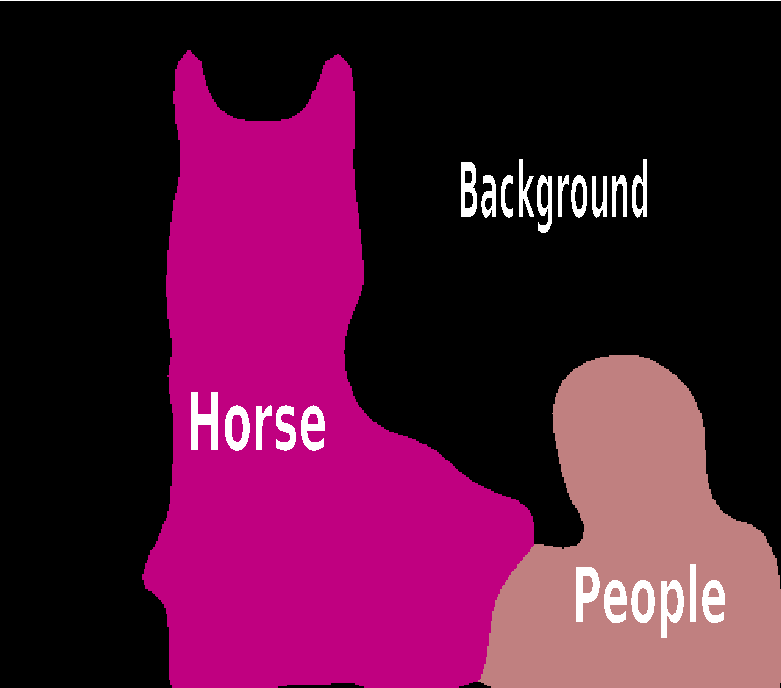
\includegraphics[width=.2\textwidth,height=.15\textwidth]{image/chap04/example/2007_000799.pdf}
		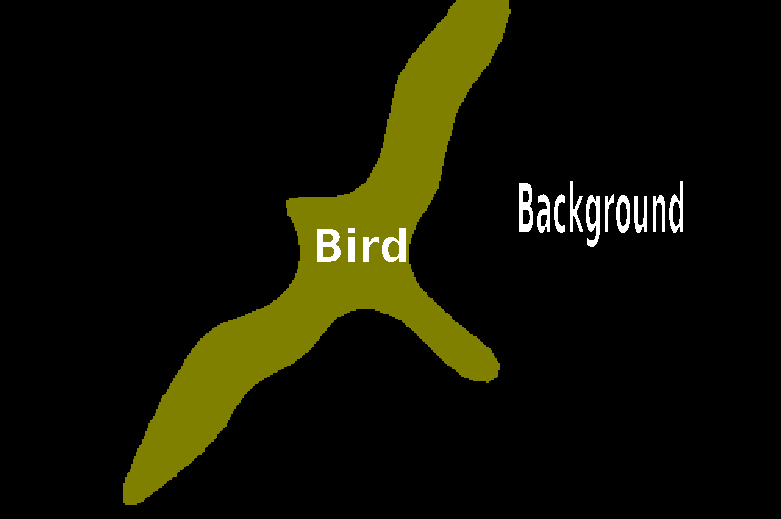
\includegraphics[width=.2\textwidth,height=.15\textwidth]{image/chap04/example/2007_002094.pdf}
		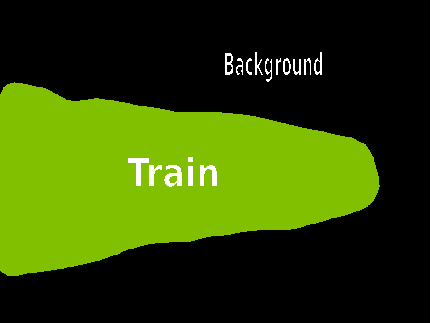
\includegraphics[width=.2\textwidth,height=.15\textwidth]{image/chap04/example/2007_004483.pdf}
		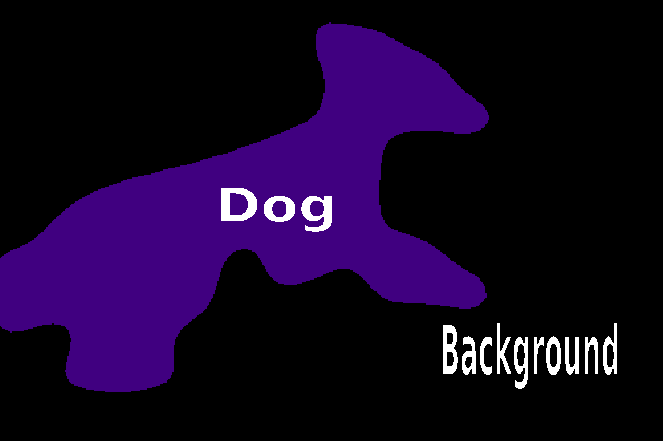
\includegraphics[width=.2\textwidth,height=.15\textwidth]{image/chap04/example/2007_003194.pdf}
		\caption[语义图像分割的例子]{本文模型在VOC 2012验证集上的语义图像分割例子}
		\label{fig:example1}
	\end{figure}
}

\frame{
	\begin{block}{选题的背景}
		\begin{itemize}
			\item 手工设计特征的局限性(SIFT, HOG)
			\item 深度学习技术的兴起
			      \begin{itemize}
				      \item 基于GPU的并行化计算
				      \item 大型训练集的标注
			      \end{itemize}
			\item 大数据与智能时代正在来临
		\end{itemize}
	\end{block}

	\begin{block}{选题的意义}
		\begin{itemize}
			\item[\dag] 图像语义分割解决了图像里面有什么,物体的形状与位置的问题
		\end{itemize}
		\vspace{-1em}
		\begin{multicols}{2}
			\begin{itemize}
				\item 图像检索
				\item 图像编辑
				\item 现实增强
				\item 机器导航
			\end{itemize}
		\end{multicols}
	\end{block}
	\}
}
\subsection*{国内外研究现状}

\frame{
	\frametitle{主流方法中的代表性工作}
	\begin{columns}[t]
		\column{.5\textwidth}
		\centering
		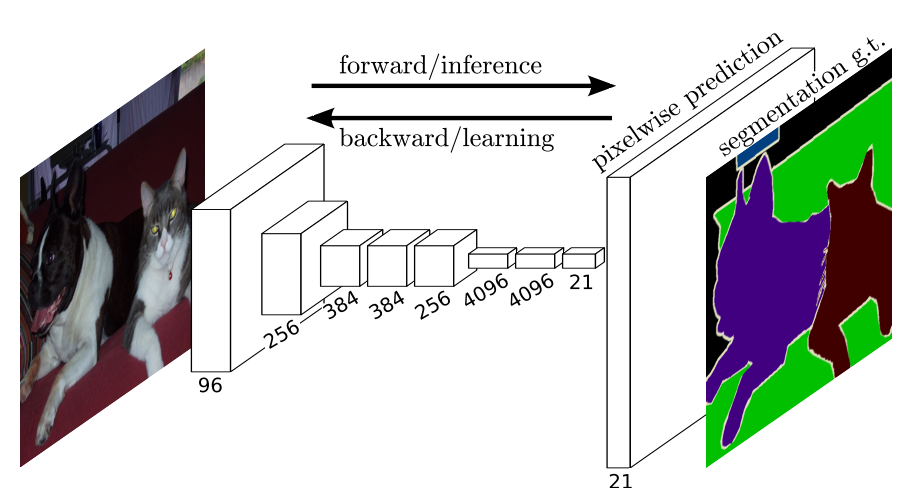
\includegraphics[width=\textwidth]{figures/FCN} \\
		\makebox[0.5\textwidth]{\tiny a. 全卷积网络[Long et al, CVPR 2015]} \\
		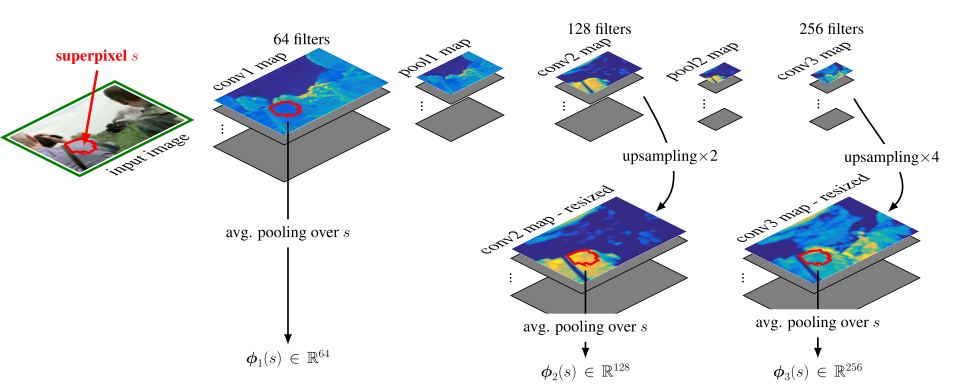
\includegraphics[width=\textwidth]{figures/zoom-out} \\
		\makebox[0.5\textwidth]{\tiny c. 卷积网络+高低层次特征融合[Mostajabi et al, CVPR 2015]}

		\column{.5\textwidth}
		\centering
		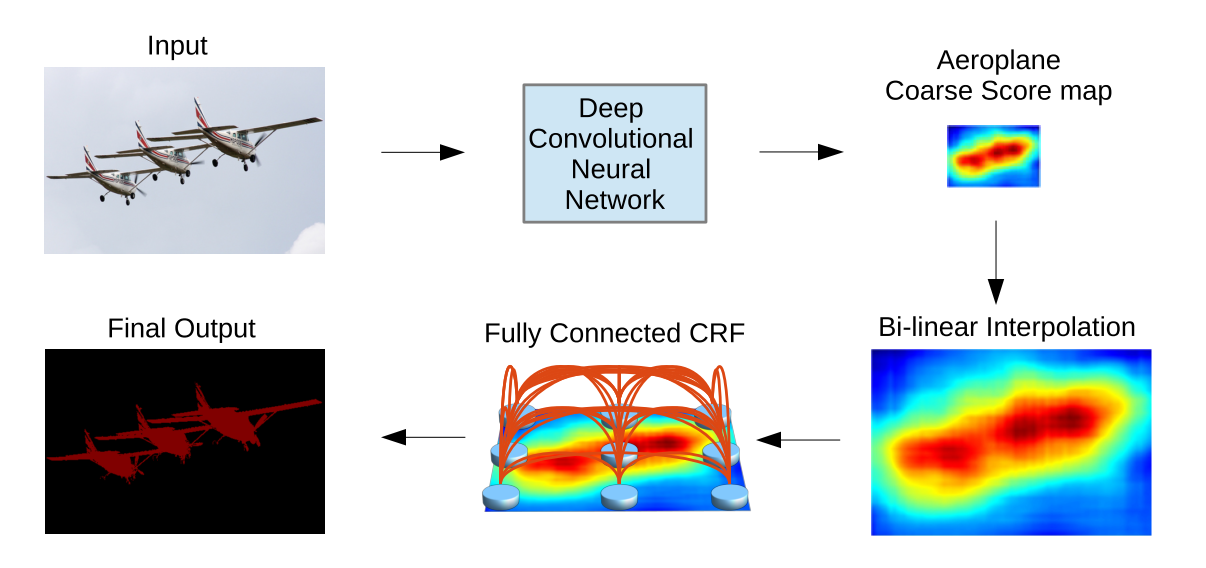
\includegraphics[width=\textwidth]{figures/Deeplab} \\
		\makebox[0.5\textwidth]{\tiny b. 全卷积网络+概率图模型[Chen et al, ICLR 2015]} \\
		\vspace{0.8em}
		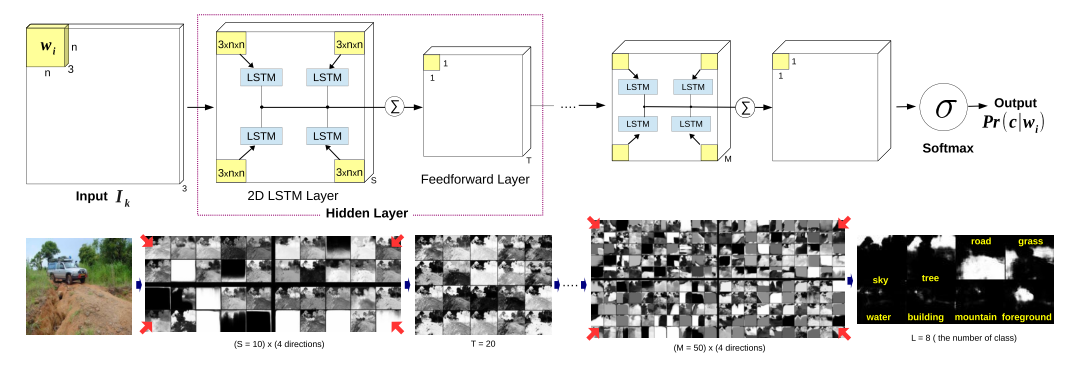
\includegraphics[width=\textwidth]{figures/LSTM} \\
		\makebox[0.5\textwidth]{\tiny d. 二维长短记忆网络[Byeon et al, CVPR, 2015]}
	\end{columns}
}
\subsection*{本文的工作}
\frame{
	\vspace{-0.6em}
	\begin{figure}[h]
		\centering
		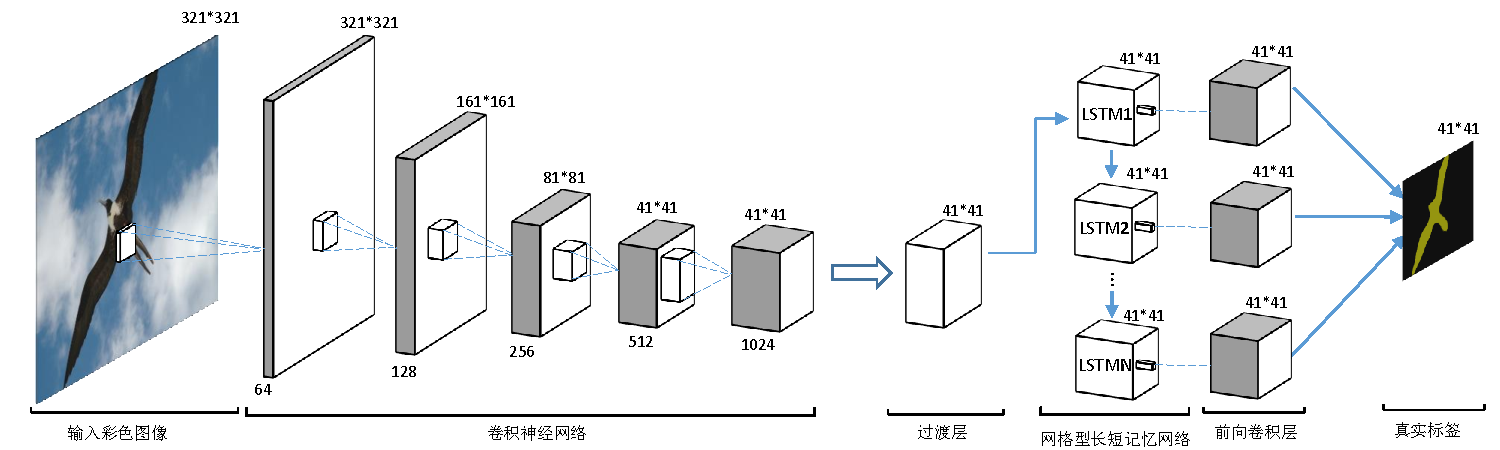
\includegraphics[width=\textwidth]{image/chap04/illustration/networkstructure.pdf}
		\caption{网络整体结构图}
	\end{figure}
	\vspace{-1.2em}
	\begin{block}{目标与思路}
		\footnotesize
		\begin{itemize}
			\item 充分利用全卷积网络强大的特征学习能力
			\item 借助长短记忆网络对特征整体与局部建模的良好能力
			\item 使用随机梯度下降法进行端到端的训练
			\item 在主流数据集验证模型有效性
		\end{itemize}
	\end{block}
}

